\chapter{Application : implémentation du projet}
\label{chap:project}

Ce chapitre relie chaque élément théorique des chapitres précédents au code du dépôt
(\texttt{text-\linebreak[1]to-\linebreak[1]image-\linebreak[1]generative-\linebreak[1]models}), une
implémentation \emph{from scratch} en PyTorch, conçue pour tourner entièrement en local sur un Mac
Apple Silicon (accélération MPS).

\section{Choix de conception}

\begin{itemize}
    \item \textbf{Diffusion pixel-space, pas latent-space.} Contrairement à Stable Diffusion, qui
    diffuse dans l'espace latent compressé d'un VAE, ce projet diffuse directement dans l'espace des
    pixels. Ce choix simplifie considérablement l'implémentation (pas de VAE à entraîner ou à
    intégrer) au prix d'une résolution de travail plus faible ($64\times64$), un compromis raisonnable
    pour un objectif pédagogique réalisable en local.
    \item \textbf{Un seul U-Net, deux approches.} Comme expliqué au chapitre~\ref{chap:architecture},
    l'architecture U-Net (\texttt{src/backend/shared/unet.py}) est strictement identique pour le DDPM
    et le flow matching : seule la construction de $x_t$ et l'interprétation de la sortie du réseau
    diffèrent.
    \item \textbf{CLIP gelé.} Le texte est encodé par \texttt{openai/clip-vit-base-patch32}
    (\texttt{transformers}), jamais réentraîné.
\end{itemize}

\section{Le jeu de données : CelebA-Dialog}

Le projet utilise CelebA-Dialog (Jiang et al., 2021) \cite{jiang2021celebadialog}, une extension de
CelebA qui associe à chacune des $202\,599$ images de visages une légende en langage naturel générée à
partir de cinq attributs à échelle graduée (\texttt{Bangs}, \texttt{Eyeglasses}, \texttt{No\_Beard},
\texttt{Smiling}, \texttt{Young}) : par exemple \og \emph{This person is a young smiling woman with
long bangs and no eyeglasses.} \fg\ Ce jeu de données permet un conditionnement textuel plus riche que
de simples labels de classe, sans nécessiter la collecte de vraies légendes humaines pour chaque
image, comme le ferait par exemple COCO Captions.

Le module \texttt{src/backend/shared/dataset.py} (classe \texttt{CelebACaptionDataset}) charge une
paire (image, légende), applique le split officiel train/val/test, et exclut automatiquement les
quelques images sans annotation disponible.

\section{Correspondance théorie $\leftrightarrow$ code}

\begin{table}[h]
\centering
\small
\begin{tabular}{@{}p{5.4cm}p{9.2cm}@{}}
\toprule
\textbf{Concept théorique} & \textbf{Fichier} \\
\midrule
Bruitage forward $q(x_t\mid x_0)$, éq.~\eqref{eq:qsample} & \texttt{src/backend/diffusion/gaussian\_diffusion.py} \newline (\texttt{GaussianDiffusion.q\_sample}) \\
Reverse process, éq.~\eqref{eq:psample} & \texttt{GaussianDiffusion.p\_sample} \\
Interpolation Flow Matching, éq.~\eqref{eq:flow-interp} & \texttt{src/backend/flow\_matching/flow\_matching.py} \newline (\texttt{ConditionalFlowMatching.sample\_xt}) \\
Encodage sinusoïdal du temps & \texttt{src/backend/shared/time\_embedding.py} \\
ResBlock, CrossAttentionBlock & \texttt{src/backend/shared/unet\_blocks.py} \\
U-Net complet & \texttt{src/backend/shared/unet.py} \\
Encodeur texte CLIP gelé & \texttt{src/backend/shared/text\_encoder.py} \\
Loss DDPM (MSE sur le bruit) et training loop & \texttt{src/backend/diffusion/train.py} \\
Loss Flow Matching (MSE sur la vélocité) et training loop & \texttt{src/backend/flow\_matching/train.py} \\
Génération par débruitage itératif (Algo. 2, chap.~\ref{chap:ddpm}) & \texttt{src/backend/diffusion/sample.py} \\
Génération par résolution ODE (Euler explicite) & \texttt{src/backend/flow\_matching/sample.py} \\
Classifier-free guidance (dropout à l'entraînement) & argument \texttt{cfg\_dropout\_prob} des deux \texttt{train.py} \\
\bottomrule
\end{tabular}
\caption{Correspondance entre les notions théoriques du cours et leur implémentation.}
\end{table}

\section{Un exemple de code : la formule fermée du bruitage}

L'équation~\eqref{eq:qsample} se traduit directement en quelques lignes de PyTorch :

\begin{lstlisting}[language=Python]
def q_sample(self, x_0, t, noise=None):
    if noise is None:
        noise = torch.randn_like(x_0)
    sqrt_alphas_cumprod_t = self._extract(self.sqrt_alphas_cumprod, t, x_0.shape)
    sqrt_one_minus_alphas_cumprod_t = self._extract(
        self.sqrt_one_minus_alphas_cumprod, t, x_0.shape
    )
    x_t = sqrt_alphas_cumprod_t * x_0 + sqrt_one_minus_alphas_cumprod_t * noise
    return x_t, noise
\end{lstlisting}

La méthode \texttt{\_extract} gère le fait que chaque image du batch peut avoir un $t$ différent
(nécessaire à l'entraînement, où $t$ est tiré aléatoirement pour chaque exemple) : elle sélectionne la
bonne valeur précalculée de $\sqrt{\bar\alpha_t}$ pour chaque élément du batch et la redimensionne pour
un broadcasting correct sur les dimensions spatiales $(H, W)$.

\section{Outils d'entraînement}

\subsection{CLI unifiée}

L'entraînement, la génération et la comparaison des deux approches passent par une CLI unique
(\texttt{python -m src.cli}), documentée en détail dans le \texttt{README.md} du dépôt :
\begin{lstlisting}[language=bash]
python -m src.cli train diffusion --epochs 5 --batch-size 32
python -m src.cli train flow_matching --epochs 5 --batch-size 32
python -m src.cli sample diffusion --checkpoint checkpoints/diffusion/latest.pt \
    --prompt "a smiling woman with bangs"
python -m src.cli compare --ddpm-checkpoint ... --flow-checkpoint ...
\end{lstlisting}

\subsection{Suivi de l'entraînement}

Deux mécanismes de suivi sont intégrés :
\begin{itemize}
    \item \textbf{TensorBoard} : chaque \texttt{train.py} logge la loss, des grilles d'images générées
    périodiquement sur un jeu de prompts fixes, et le temps par epoch, dans le dossier
    \texttt{tensorboard/} propre à chaque approche (sous \texttt{checkpoints/}).
    \item \textbf{Page de monitoring live} (frontend React, onglet \og Suivi entraînement \fg) : une
    API FastAPI (\texttt{src/frontend/api/main.py}, endpoint \texttt{/training-status}) lit ces mêmes
    logs TensorBoard directement depuis le disque et les expose à une page web qui se rafraîchit
    automatiquement, sans dépendre de TensorBoard lui-même.
\end{itemize}

\begin{figure}[h]
\centering
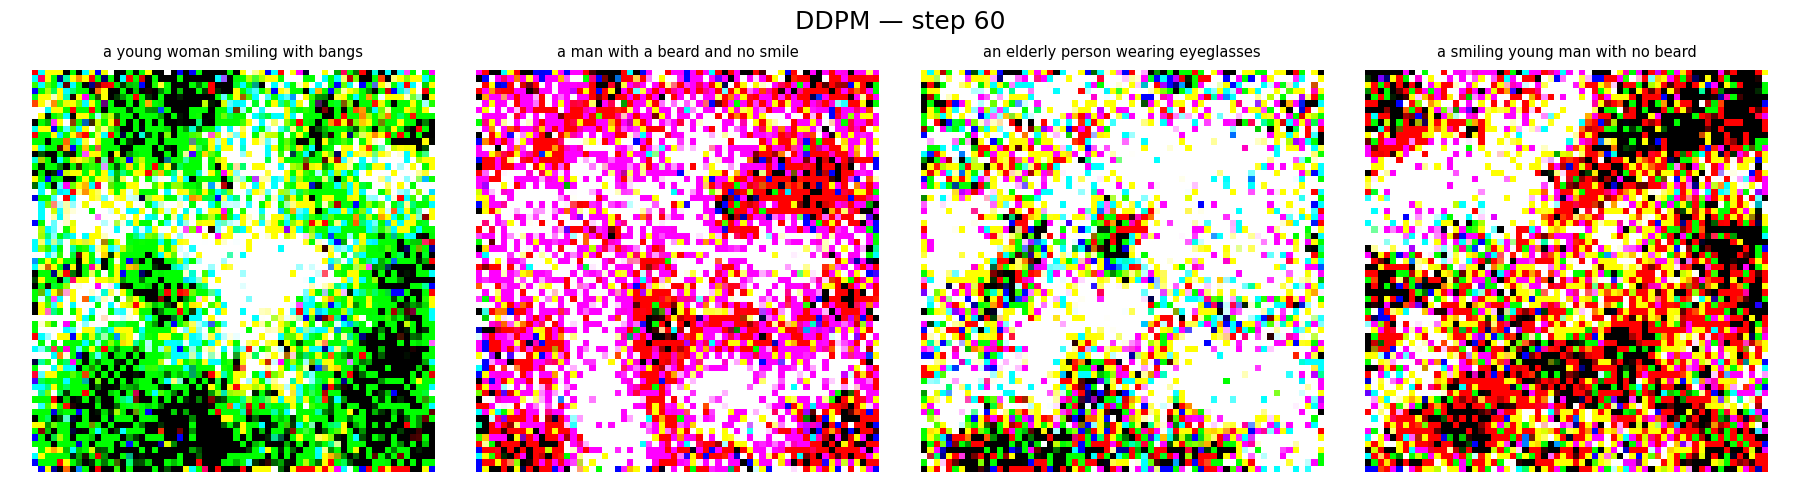
\includegraphics[width=0.85\textwidth]{figures/early_training_preview.png}
\caption{Exemple de grille de preview générée automatiquement pendant l'entraînement (ici après
seulement 60 pas d'optimisation, à titre d'illustration du mécanisme de suivi — le modèle n'a pas
encore convergé et ne produit que du bruit structuré ; un entraînement complet de plusieurs epochs est
nécessaire pour obtenir des visages reconnaissables).}
\label{fig:early-preview}
\end{figure}

\section{Interface de génération}

Un frontend web (React + Vite) et une API FastAPI permettent de générer des images depuis un
navigateur, en choisissant l'approche (DDPM ou Flow Matching), le prompt et le nombre d'étapes de
sampling. Les modèles sont chargés paresseusement par l'API (au premier appel), ce qui permet de
démarrer le serveur sans qu'aucun modèle ne soit encore entraîné.
